DARWIN is a high-level description of an algorithm, that can be used to solve
a~multi-objective optimization problem. It is a~list steps to execute and
calculations to perform. Therefore, one does not need a computer to realize
the decision-making process. However, in practise it is almost impossible to
complete all the steps without a dedicated software application. Moreover, to
evaluate the method's performance one needs to repeat the experiments many
times over and over again.

For the reasons stated above it was required to implement the method on a
computer system. This chapter describes technologies used for the DARWIN's
implementation and an experiment framework development.

\section{The method's implementation}

The environment, in which DARWIN has to function is not empty; thus has to be
taken into account during the development of the implementation. It is shown
in~fig.~\ref{environ}. Darwin is a~realisation of an interactive process,
therefore a way of complication with the decision maker is required. Another
restriction is imposed by the need of inducing decision rules from the sorted
examples of solutions.

The DM has to provide a problem he wants to solve. It can be done in a model
file. If one wants to change the default parameters' values a~configuration
file with the values is also required. Moreover, during the algorithm run,
presence of the decision maker is required, in order to select ``good''
solutions from the provided ones. Consult the user manual ([inref]) for more
details on the file formats. The parameters are described later in this
section.

Decision rules store the decision maker preferences, therefore they are
a~symbolic representation of trade-offs he or she is willing to make, as well
as the importance of each criterion. They are ensuring a~robustness of the
resulting solutions because of an underlying DRSA framework. Te rules are
a~very important part of the method. Thus, a~way --- an algorithm --- to
generate them is need. In the method description a~phase of obtaining the
rules is treated as a~black-box. It is assumed that a~component able to
generate rules from the DM's selection exists.



\begin{figure}
  \centering 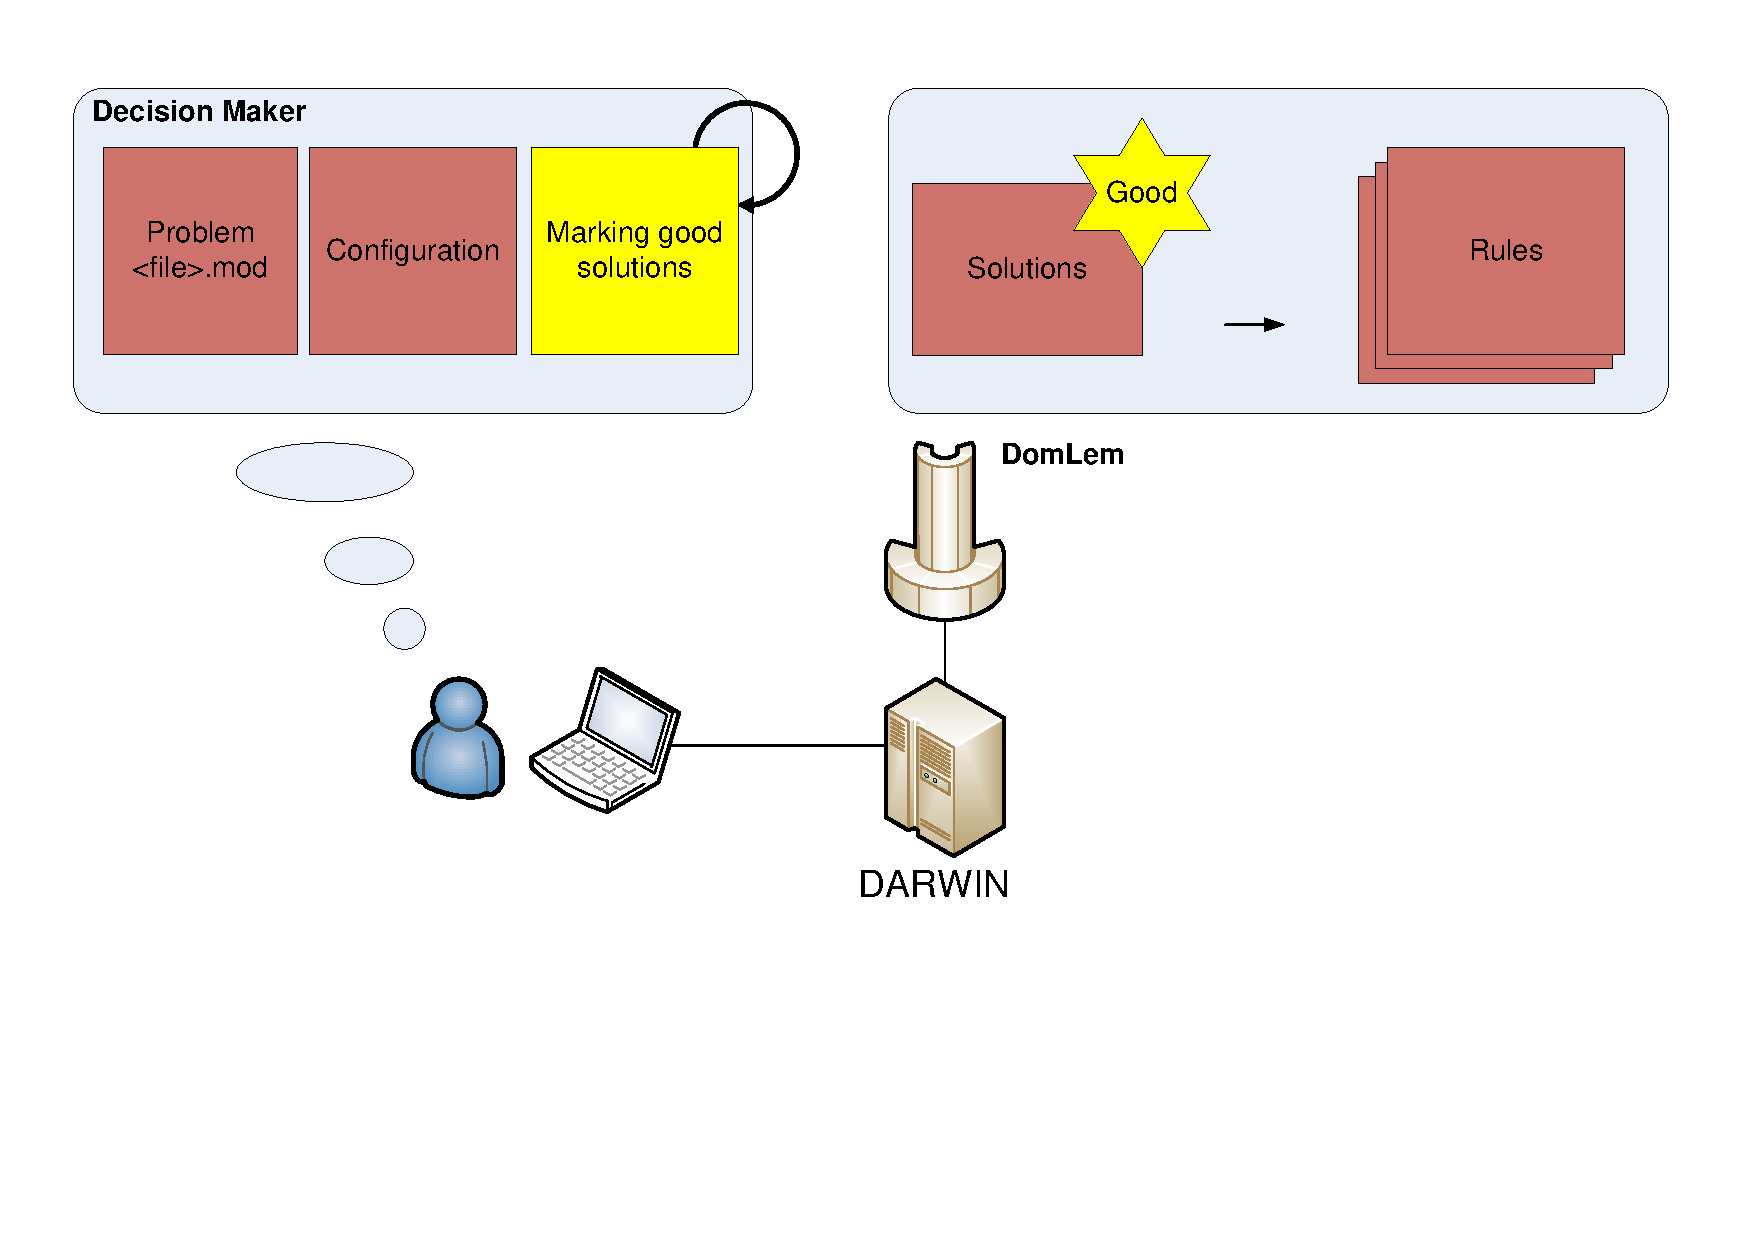
\includegraphics[scale=0.5]{img/environ}
  \caption{DARWIN's environment}
  \label{environ}
\end{figure}

\section{Experiment framework}
